% !TEX TS-program = pdflatex

\documentclass[unicode,11pt,notheorems,xcolor=table]{beamer}

\usepackage[T2A]{fontenc}
\usepackage[utf8]{inputenc}
\usepackage[russian]{babel}
\usepackage{amsmath,amsfonts,amssymb,amsthm}
\usepackage{mathtools}
\usepackage{diagbox}

\usepackage{ulem}
\usepackage{tikz, graphicx}
%\usepackage{tkz-graph}
\usetikzlibrary{matrix,arrows,decorations.pathmorphing, arrows.meta,positioning}
\usetikzlibrary{positioning,calc}
\usetikzlibrary{petri}
\usetikzlibrary{decorations.pathreplacing}

%Описание стиля презентации
\usetheme[sidebar=0]{kfmn} 
\setbeamercovered{transparent}

%\definecolor{cyan}{RGB}{240,217,1}
%\definecolor{vgugreen}{RGB}{143,188,103}
%\definecolor{vgured}{RGB}{234,38,40}
%\definecolor{vgublue}{RGB}{53,101,167}



\makeatletter
	\g@addto@macro{\endtabular}{\rowfont{}}% Clear row font
	\makeatother
	\newcommand{\rowfonttype}{}% Current row font
	\newcommand{\rowfont}[1]{% Set current row font
		\gdef\rowfonttype{#1}#1\ignorespaces%
	}
\makeatother

\newcommand{\myunit}{9mm}
\tikzset{
    node style sp/.style={draw,circle,minimum size=\myunit},
    node style ge/.style={circle,minimum size=\myunit},
    arrow style mul/.style={draw,sloped,midway,fill=white},
    arrow style plus/.style={midway,sloped,fill=white},
}

%[0, 6, 8, 8, 10, 5, 6, 10, 8, 10, 10], 

\pgfdeclareimage[height=8mm]{university-logo}{logo-iem.png}
\logo{\pgfuseimage{university-logo}}
%2[0, 11, 10, 8, 11, 5, 11, 11, 8, 11, 10, 11],

\titlepicture{
	\begin{tikzpicture}[y=1.4cm,overlay,rotate=8]
	\coordinate (O) at (-3cm,0.9cm);
	\filldraw[thick,draw= vgublue, fill=vgublue!20!white] (0,0) circle[radius=4.2cm];
	\clip (0,0) circle[radius=4.2cm];
	\draw (-1.5,1.5) node{
	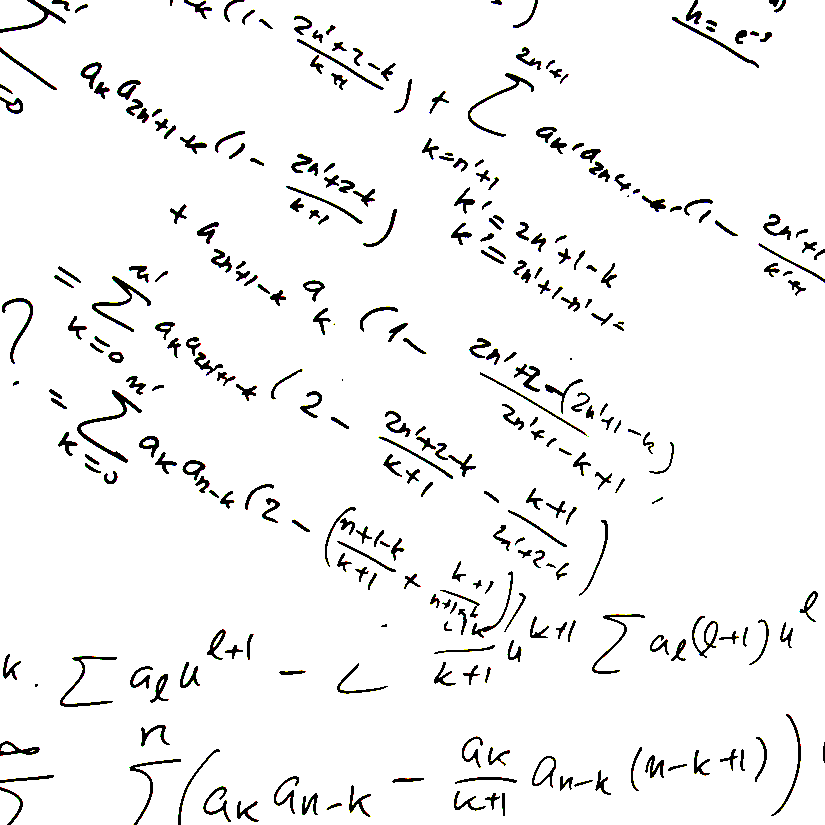
\includegraphics[width=8cm]{titlepic.png}
	};
\end{tikzpicture}
}

\usepackage[math]{iwona}

\newcommand{\hplus}{\mathbin{\hat+}}
\newcommand{\hdot}{\mathbin{\hat\cdot}}
% Описание теорем
\newtheorem{theorem}{Теорема}
\newtheorem{seq}{Следствие}
%%

\LECT % 

% Титульный лист теорем
\author[Д.\,В. Чупраков]{канд.\,физ.-матем.\,наук, доцент Д.\,В. Чупраков\\[6pt] usr10381@vyatsu.ru}

\institute[ВятГУ]{ФГБОУ ВО Вятский государственный университет}

\department{Факультет экономики и финансов}

\title[Лекция~8. Балансовые модели]{
	Введение в экономико-математическое моделирование\\[12pt]
	Лекция~8. Балансовые модели}
%\subtitle{Теория двойственности и транспортная задача}

\date{28 октября 2020~г.}


\setbeamercovered{invisible}



\begin{document}


\maketitle

\begin{frame}{Структура лекции}
	\tableofcontents
\end{frame}



\section{О балансовых моделях}
\begin{frame}{Понятие балансовой модели}{}
	\begin{block}{Определение}
		\alert{Балансовая модель}~--- система уравнений, каждое из которых выражает требование баланса между производимым отдельными экономическими объектами количеством продукции и совокупной потребностью в этой продукции. 	
	\end{block}
    

	\begin{itemize}
		\item  
		система состоит из объектов,
		\item  
		каждый объект выпускает некоторый продукт, 
		\item 
		часть продукта потребляется другими объектами системы, 
		\item 
		часть выводится за пределы системы в качестве конечного продукта. 
	\end{itemize}
\end{frame}
% Балансовые модели, как статические, так и динамические, широко применяются при экономико-математическом моделировании экономических систем и процессов. 

\begin{frame}{Балансовый метод}
    \alert{Балансовое соответствие}~--- равенство объемов запаса ресурсов и величины потребности в нем.

	\structure{Примеры:}
	\begin{itemize}
		\item наличие рабочей силы~--- количества рабочих мест
		\item платежеспособный спроса населения~--- предложение товаров и услуг
	\end{itemize}
	\begin{block}{Определение}
		\alert{Балансовый метод}~--- метод взаимного сопоставления имеющихся материальных, трудовых и финансовых ресурсов и потребностей в них.
	\end{block}

\end{frame}


\begin{frame}{Область и границы применения}
	\structure{Область применения:}

	Балансовый метод~--- основной инструмент поддержания пропорций в народном хозяйстве. 

	\bigskip
	\structure{Границы применения:}
		\begin{itemize}
		\item
			не имеют механизмов сравнения отдельных вариантов экономических решений 
		\item 
			не предусматривают взаимозаменяемости ресурсов, 
		\item 
			не позволяют сделать выбор оптимального варианта развития экономической системы.
	\end{itemize}
\end{frame}


\begin{frame}{Виды балансовых моделей}
\begin{itemize}
	\item межотраслевые балансы;
	\item частные материальные, трудовые и финансовые балансы;
	\item матричные финансовые планы предприятий;
\end{itemize}

\begin{block}{}
	Все модели имеют общий принцип построения и системы расчетов.
\end{block}
\end{frame}

\section{Модель межотраслевого баланса}

\begin{frame}{Модель межотраслевого баланса}
\alert{Межотраслевой баланс} (МОБ)~--- каркасная модель
экономики:
	\begin{itemize}
		\item отражает натуральные и стоимостные связи;
		\item дает комплексную характеристику процесса формирования и использования совокупного продукта в отраслевом разрезе.
	\end{itemize}
\end{frame}
\begin{frame}{Основные предположения МОБ}
	\begin{itemize}
		\item каждая отрасль производит только один продукт;
		\item каждая отрасль имеет только одну технологию производства продукции, которая характеризуется коэффициентами затрат;
		\item коэффициенты затрат отражают взаимосвязь между отраслями и являются отраслевыми нормативами затрат.
	\end{itemize}
\end{frame}

\begin{frame}[allowframebreaks]{Основные обозначения МОБ}
	\begin{itemize}
		\item \structure{$X_i$}~--- валовой выпуск продукции $i$-й отрасли за рассматриваемый промежуток времени;
		\item \structure{$Y_i$}~---  конечное потребление,~--- объем продукции отрасли~$i$, потребляемый в непроизводственной сфере:
		\begin{itemize}
			\item личное потребление
			\item обеспечение общественных потребностей
			\item экспорт
		\end{itemize}
		\item \structure{$Z_j$}~--- Условно-чистая продукция $j$-й отрасли:
		\begin{itemize}
			\item чистый доход
			\item сумма оплаты труда
			\item сумма амортизации
		\end{itemize}

		\framebreak		
		\item \structure{$x_{ij}$}~--- межотраслевые потоки продукции,~--- объем продукции отрасли $i$, расходуемый отраслью~$j$;
		\item \structure{$x_{ii}$}~--- внутреннее потребление $i$-ой отрасли;
		\item $\sum\limits_{i=1}^n x_{ij}$~--- производственные затраты $j$-й отрасли на приобретение продукции других отраслей;
		\item $\sum\limits_{j=1}^n x_{ij}$~--- сумма всех поставок $i$-й 		
		\item $\sum\limits_{i=1}^n\sum\limits_{j=1}^n x_{ij}$~--- промежуточный продукт экономики;
	\end{itemize}
\end{frame}

\subsection{Общая таблица межотраслевого баланса}
\begin{frame}{Таблица межотраслевого баланса}
	 \scriptsize

	 ~\hspace{-9.5mm}
	 \begin{tabular}{|c|>{\columncolor{red!20}}c|>{\columncolor{red!20}}c|>{\columncolor{red!20}}c|>{\columncolor{red!20}}c|>{\columncolor{red!20}}c||>{\columncolor{yellow!30}}c|>{\columncolor{yellow!30}}c|}
		\hline
		\rowcolor{white}
	 	Производящие& \multicolumn{4}{p{2cm}|}{Потребители}& Промежут. & Конечное  & Валовой\\
		 \rowcolor{white}
		 отрасли &  1& 2& $\cdots$ & n & потребление & потребление & продукт\\
		  \hline
		  1 & $x_{11}$ & $x_{12}$ & $\cdots$ & $x_{1n}$ & $\sum\limits_{j=1}^n x_{1j}$ & $Y_1$ & $X_1$\\
		  \hline
		  2 & $x_{21}$ & $x_{22}$ & $\cdots$ & $x_{2n}$ & $\sum\limits_{j=1}^n x_{2j}$ & $Y_2$ & $X_2$\\
		  \hline
		  $\cdots$ & $\cdots$ & $\cdots$ & $\cdots$ & $\cdots$ & $\cdots$ & $\cdots$ & $\cdots$ \\
		  \hline
		  n & $x_{n1}$ & $x_{n2}$ & $\cdots$ & $x_{nn}$ & $\sum\limits_{j=1}^n x_{nj}$ & $Y_n$ & $X_n$\\
		  \hline
		  \multicolumn{1}{|p{1.3cm}|}{\centering Промежут. затраты} & $\sum\limits_{i=1}^n x_{i1}$ & $\sum\limits_{i=1}^n x_{i2}$ & $\cdots$ & $\sum\limits_{i=1}^n x_{in}$ & $\sum\limits_{i=1}^n\sum\limits_{j=1}^n x_{ij}$ & $\sum\limits_{i=1}^n Y_{i}$ & $X_n$\\
		  \hline
		  \hline
		  \rowcolor{blue!20} 
		  \multicolumn{1}{|p{1.5cm}|}{\cellcolor{white}\centering Условно-чистая продукция} & $Z_1$ & $Z_2$ & $\cdots$ & $Z_n$ & $\sum\limits_{j=1}^n Z_j$ & \cellcolor{green!20} $\sum\limits_{j=1}^n Z_j=\sum\limits_{i=1}^n Y_i$ & \cellcolor{green!20} ~\\
		  \hline
		  \rowcolor{blue!20} 
		  \multicolumn{1}{|p{1.5cm}|}{\cellcolor{white}\centering Валовой продукт} & $X_1$ & $X_2$ & $\cdots$ & $X_n$ &  & \cellcolor{green!20}  & \cellcolor{green!20} $\sum\limits_{j=1}^n X_j$\\
		  \hline
		\end{tabular}
\end{frame}


\begin{frame}{Квадратны таблицы}
	\begin{itemize}
		\item 
			\structure{I~квадрант}~--- таблица межотраслевых взаимосвязей. 
		\item 
			\structure{II~квадрант}~--- материально-вещественный состав конечной продукции.
		\item 
			\structure{III~квадрант}~--- стоимостной состав конечной продукции.
		\item 
			\structure{IV~квадрант}~--- конечное распределение и использование национального дохода. 
	\end{itemize}
\end{frame}


\subsection{Соотношения межотраслевого баланса}

\begin{frame}{Основные соотношения МОБ}
	\begin{itemize}
		\item Распределение продукции отраслей по направлениям использования:
		$$	
			X_i = \sum_{j=1}^n x_{ij}+Y_i, \qquad i =\overline{1,n}
		$$
		\item Стоимостной состав продукции:
		$$
			X_j = \sum_{i=1}^n x_{ij}+Z_j, \qquad j = \overline{1,n}	
		$$
	\end{itemize}
\end{frame}


\begin{frame}{}
	\begin{block}{Tеорема}
		\itshape
		В МОБ соблюдается принцип единства материального и~стоимостного составов национального дохода:
	$$
		\sum_{i=1}^n Y_i = \sum_{j=1}^n Z_j
	$$
	\end{block}
	\pause
	Действительно:	
	$$
	\only<3->{\alert{-} \left.}
	\begin{aligned}
		\sum_{i=1}^n X_i &= \sum_{i=1}^n\sum_{i=1}^n x_{ij}+\sum_{i=1}^n Y_i\\
		\sum_{j=1}^n X_j &= \sum_{j=1}^n\sum_{i=1}^n x_{ij}+\sum_{j=1}^n Z_j
	\end{aligned}
	~\only<3->{\right|}
	\only<3->{\Rightarrow \alert{\sum_{i=1}^n Y_i - \sum_{j=1}^n Z_j=0 }}
	$$

	
\end{frame}

\begin{frame}{}
Выделяют два вида моделей межотраслевого баланса:
\begin{enumerate}
	\item \structure{модель отчетного МОБ:}
	$$	
		X_i = \sum_{j=1}^n x_{ij}+Y_i, \qquad X_j = \sum_{i=1}^n x_{ij}+Z_j,
	$$
	\item \structure{модель прогнозного  МОБ:}
	$$
		X_i = \sum_{j=1}^n x_{ij}+Y_i
	$$
\end{enumerate}
\begin{block}{}
	Модель прогнозного межотраслевого баланса также называется моделью «затраты --- выпуск» В.~Леонтьева.	
\end{block}	

\end{frame}
\section{Статическая модель межотраслевого баланса В.~Леонтьева}
\begin{frame}{Василий Васильевич Леонтьев (1906--1999)}

	\begin{minipage}{35mm}
		\noindent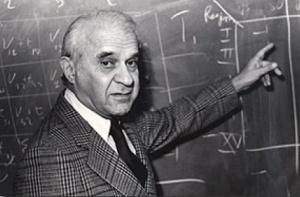
\includegraphics[width=35mm]{Leontyev.jpg}
	\end{minipage}
	\begin{minipage}{70mm}
		\structure{Лауреат  Премии Шведского национального банка по экономическим наукам памяти А. Нобеля (1973) «за развитие метода ,,затраты — выпуск`` и за применение этого метода в~основных проблемах экономики»}
	\end{minipage}

	\medskip
{\small	
\begin{itemize}
	\item 1936~---Впервые сформулирована проблема расчета связи между отраслями через выпуск и потребление  продукции разного вида.
	\item 1941~--- ,,Структура Американской экономики, 1919--1939``
	\item 1953~--- ,,Исследования структуры американской экономики``
	\item 1966~--- ,,Экономическая теория затраты-выпуск``
	\item 1977~--- ,,Будущее мировой экономики`` 
	\item 1977~--- ,,Очерки по экономике``
\end{itemize}\par}
\end{frame}	
\begin{frame}{Исходные посылки модели Леонтьева}
	\begin{itemize}
		\item Экономика состоит из  взаимосвязанных отраслей.
		\item Каждая отрасль выпускает только один вид продукта.
		\item Каждый продукт производится только одной отраслью.
		\item В каждой отрасли имеется единственная технология производства; не допускается замещение одного ресурса другим.
		\item \alert{Взаимосвязь между выпуском продукции отраслей и затратами описывается линейными уравнениями.}
	\end{itemize}
\end{frame}

	\begin{frame}{Условие линейности прямых затрат}
	\begin{block}{Определение}
		\alert{Коэффициент прямых материальных затрат $a_{ij}$}~---  количество продукции $i$-й отрасли, которое требуется  предоставить $j$-й~отрасли для производства единицы продукции. 
		$$
			\alert{a_{ij}= \frac{x_{ij}}{X_j}}
		$$
	\end{block}

	\structure{Экономический смысл}
	Затраты $i$-ой отрасли в $j$-ую линейно зависят от валового выпуска $X_j$. 
	
\end{frame}

\subsection{Технологическая матрица (матрица полных затрат)}

\begin{frame}{Технологическая матрица}

	\begin{block}{}
		$$
		A= \begin{pmatrix}
			a_{11} & a_{12} &\cdots & a_{1n}\\
			a_{21} & a_{22} &\cdots & a_{2n}\\
			\cdots & \cdots & \cdots & \cdots\\
			a_{n1} & a_{n2} &\cdots & a_{nn}\\
		\end{pmatrix}
		$$
	\end{block}
	\structure{Свойства технологической матрицы:} 
	\begin{enumerate}
		\item Неотрицательность, $a_{ij}\geqslant 0$. 
		\item Диагональные элементы $a_{ii}\leqslant 1$. 
		\item Сумма элементов матрицы $A$ по любому из столбцов не превосходит 
		единицы.
	\end{enumerate}
\end{frame}


\begin{frame}{Математическая модель Леонтьева}
	\structure{Распределение продукции по направлениям использования:}
	$$
		X_i = \sum_{j=1}^n x_{ij} +Y_i = \sum_{j=1}^n a_{ij}X_j + Y_j
	$$
	
	\bigskip
	\begin{block}{Модель в форме СЛУ}
	$$
		\left\lbrace
		\begin{aligned}
			X_1 &= a_{11}X_1 +  a_{12} X_2  + \ldots + a_{1n}X_n  + Y_1\\
			X_2 &= a_{21}X_1 +  a_{22} X_2  + \ldots + a_{2n}X_n  + Y_2\\
			&\cdots\\
			X_n &= a_{n1}X_1 +  a_{n2} X_2  + \ldots + a_{nn}X_n  + Y_n\\
		\end{aligned}
		\right.
	$$
	\end{block}
\end{frame}

\begin{frame}{Матричная форма модели Леонтьева}
	$$ 
		X = \begin{pmatrix}
			X_{1} \\ X_{2} \\\cdots\\ X_{n}
		\end{pmatrix},
		\qquad
		Y = \begin{pmatrix}
			Y_{1} \\ Y_{2} \\\cdots\\ Y_{n}
		\end{pmatrix},	
		\qquad
		A= \begin{pmatrix}
			a_{11} & a_{12} &\cdots & a_{1n}\\
			a_{21} & a_{22} &\cdots & a_{2n}\\
			\cdots & \cdots & \cdots & \cdots\\
			a_{n1} & a_{n2} &\cdots & a_{nn}\\
		\end{pmatrix}
	$$
	$$
	\alert{X=AX+Y}		
	$$
	
	
	\bigskip
	\begin{block}{Связь производства и конечного потребления}
		$$
			Y=(A-E)X,\qquad  X=(A-E)^{-1}Y
		$$
			
	\end{block}

\end{frame}
\begin{frame}{Коэффициенты полных затрат}
	\structure{Матрица полных затрат}
	$$
		\alert{B = (E - A)^{-1}}
	$$
	
	% \medskip
	\structure{Экономический смысл:}

	\alert{Коэффициент полных материальных затрат $b_{ij}$}~--- величина валового выпуска продукции $i$-й отрасли, необходимого для обеспечения выпуска единицы конечного продукта $j$-й отрасли.

	\bigskip
	\structure{Основная задача межотраслевого баланса:}
	определить, как скажется на валовом выпуске каждой отрасли предполагаемое изменение объемов конечной продукции всех отраслей:
	$$
		\Delta X = (E-A)^{-1}\Delta Y
	$$
\end{frame}
\begin{frame}[allowframebreaks]{Пример}{}
	Дана неполная балансовая таблица:
	{\centering
	\begin{tabular}{cccc}
		\hline
		Производство & \multicolumn{2}{c}{Потребление} & Валовой\\
		  &  1 &   2 & выпуск\\
		\hline
		1 &  26& 164 & 260\\
		2 & 208&  82 & 410\\
		\hline
	\end{tabular}
	\par}

	\medskip
	\structure{Задачи:}
	\begin{enumerate}
		\item определить объем конечной продукции.
		\item найти объем валового выпуска каждой отрасли, если в плановом периоде выпуск конечной продукции должен повысится в 1-ой отрасли на 50\%, во 2-ой отрасли на 20\%,
	\end{enumerate}
	\framebreak

	\structure{Найдем объем конечной продукции.}
	
	Вычтем из валового продукта расходы на внутренние расходы
	$$Y= 
		\begin{pmatrix}
			Y_1\\ Y_2
		\end{pmatrix}
	 	= 
		\begin{pmatrix}
			260\\ 410
		\end{pmatrix} 
		- 
		\begin{pmatrix}
			26\\ 208
		\end{pmatrix}
		-
		\begin{pmatrix}
			164 \\ 82
		\end{pmatrix}
		=
		\begin{pmatrix}
			70\\ 120
		\end{pmatrix}
	$$
	\bigskip
	{\centering
	\begin{tabular}{ccccc}
		\hline
		Производство & \multicolumn{2}{c}{Потребление}  &Конечное & Валовой\\
		  &  1 &   2 & потребление &выпуск\\
		\hline
		1 &  26& 164 &70& 260\\
		2 & 208&  82 &120& 410\\
		\hline
	\end{tabular}
	\par}

	\framebreak

	
	В плановом периоде выпуск конечной продукции должен повысится в 1-ой отрасли на 50\%, во 2-ой отрасли на 20\%,
	Таким образом, 
	$$
		Y_{\text{план.}}
		= 
		\begin{pmatrix}
			1.5Y_1\\ 1.2Y_2 
		\end{pmatrix}
		= 
		\begin{pmatrix}
			105\\ 144 
		\end{pmatrix}
	$$
	\structure{Найдем требуемый объем выпуска}
	\begin{itemize}
		\item Составим технологическую матрицу:
			$$
				A 
				= \begin{pmatrix}
					x_{11}/X_1 & x_{12}/X_2 \\
					x_{21}/X_1 & x_{22}/X_2 \\
				\end{pmatrix}
				= \begin{pmatrix}
					26/260 & 164/410 \\
					208/260 & 82/410 \\
				\end{pmatrix}
				= \begin{pmatrix}
					0.1 & 0.4 \\
					0.8 & 0.2 \\
				\end{pmatrix}
			$$
		\item Запишем уравнение модели Леонтьева:
			$ AX+Y=X$ и выразим $X=(E-A)^{-1}Y$
			$$
			E-A 
			= \begin{pmatrix}
				1 & 0 \\
				0 & 1 \\
			\end{pmatrix}
			-
			\begin{pmatrix}
				0.1 & 0.4 \\
				0.8 & 0.2 \\
			\end{pmatrix}
			=
			\begin{pmatrix}
				 0.9 & -0.4 \\
				-0.8 & 0.8 \\
			\end{pmatrix}
			$$
		\item  Найдем обратную матрицу:
		\begin{multline*}
		(E-A)^{-1}= \frac{1}{\det(E-A)} \begin{pmatrix}
			\mathcal{A}_{11} & \mathcal{A}_{12}\\ 
			\mathcal{A}_{21} & \mathcal{A}_{22}\\ 
		\end{pmatrix}^T
		=\\
		= \frac{1}{0.4} 
		\begin{pmatrix}
			0.8 & 0.8\\ 
			0.4 & 0.9\\ 
		\end{pmatrix}^T
		= \frac{1}{0.4} 
		\begin{pmatrix}
			0.8 & 0.4\\ 
			0.8 & 0.9\\ 
		\end{pmatrix} 
		= 	
		\begin{pmatrix}
			2 & 1\\ 
			2 & 2.25\\ 
		\end{pmatrix} 
		\end{multline*}
	\item Итак, 
	$$
	X_\text{план.} = (E-A)^{-1} Y_\text{план.} = 
		\begin{pmatrix}
			2 & 1\\ 
			2 & 2.25\\ 
		\end{pmatrix} \cdot
		\begin{pmatrix}
			105\\ 144 
		\end{pmatrix}
		=
		\begin{pmatrix}
			354\\ 534 
		\end{pmatrix}
	$$
\end{itemize}
\framebreak
\structure{Плановый баланс:}
{\centering
	\begin{tabular}{ccccc}
		\hline
		Производство & \multicolumn{2}{c}{Потребление}  &Конечное & Валовой\\
		  &  1 &   2 & потребление &выпуск\\
		\hline
		1 &  26& 164 &105& 354\\
		2 & 208&  82 &144& 534\\
		\hline
	\end{tabular}
	\par}
\end{frame}

\subsection{Продуктивность  модели Леонтьева }
\begin{frame}{Продуктивность матрицы прямых затрат}
	\begin{block}{Определение}
		Неотрицательную матрицу $A$ называют \alert{продуктивной}, если существует такой неотрицательный вектор
		$X \geqslant 0$, что $X > AX$.		
	\end{block}
	
	\bigskip
	\structure{Экономический смысл:}

	Матрица $A$ продуктивная тогда и только тогда, когда существует неотрицательный ненулевой вектор конечной продукции~$Y$ для модели межотраслевого баланса. 
	
\end{frame}

\begin{frame}{Условия продуктивности}
	\begin{theorem}[Первый критерий продуктивности]
		Чтобы матрица~$A$ была продуктивной, необходимо и достаточно, 		чтобы  существовала матрица $(E - A)^{-1} \geqslant 0$
	\end{theorem}

	\vspace{1cm}
	\begin{theorem}[Второй критерий продуктивности]
		Матрица~$A$ продуктивна тогда и только тогда, когда суммы элементов каждого столбца не превосходят 1, причем существует столбец, сумма элементов которого строго меньше 1.
	\end{theorem}
\end{frame}
\begin{frame}{Пример}
	Убедимся, что технологическая матрица из предыдущего примера продуктивная
	$$
	A=\begin{pmatrix}
		0.1 & 0.4\\ 
		0.8 & 0.2\\ 
	\end{pmatrix} 
	$$
	
	Действительно 
	\begin{itemize}
		\item $0.1+0.8 < 1$, 
		\item $0.4+0.2 < 1$
	\end{itemize}
	

	По второму критерию матрица продуктивна.

\end{frame}
\subsection{Косвенные затраты}

\begin{frame}{Косвенные затраты}
	\alert{Косвенные затраты}~--- это затраты, которые входят в данный продукт не непосредственно (как прямые затраты), а через затраты других
	отраслей. 
	
	\medskip
	\structure{Обозначение:} $A^{(k)}$~--- матрица коэффициентов косвенных материальных затрат $k$-го порядка. 
	
	\medskip
	\structure{Вычисление:}
	$$
		A^{(1)}=A^2,
		\qquad 
		A^{(2)}=A^{(1)}A=A^3,
		\qquad 
		\ldots,
		\qquad 
		\alert{A^{(k)} = A^{k-1}}
	$$
	

	\begin{block}{}
	Полные затраты на выпуск единицы продукции могут быть получены, как сумма прямых и всех косвенных затрат плюс единица продукции которая выходит за сферу производства
	
	$$
		B= E+A+A^2+A^3+\ldots + A^k+ \ldots
	$$
	\end{block}
\end{frame}

\begin{frame}{Пример}
	Найдем косвенные затраты первого порядка:
	$$
	A^{(1)} = A^2 = 
	\begin{pmatrix}
		0.1 & 0.4\\ 
		0.8 & 0.2\\ 
	\end{pmatrix} 
	\cdot
	\begin{pmatrix}
		0.1 & 0.4\\ 
		0.8 & 0.2\\ 
	\end{pmatrix} 
	=
	\begin{pmatrix}
		0.33 & 0.09\\ 
		0.24 & 0.36\\ 
	\end{pmatrix} 
	$$
\end{frame}

\section{О динамических моделях межотраслевого баланса}
\begin{frame}{Динамические модели МОБ}
	\structure{Цель:} установить взаимосвязь между предыдущими и последующими этапами развития экономики.

	\medskip
	\structure{В основе модели:} зависимость между величиной капитальных вложений и приростом продукции.

	\medskip
	\structure{Уравнение распределения}
	$$
		X_i 
		= \sum_{j=1}^n x_{ij} 
		\only<2->{\alert{{}+ \sum_{j=1}^n \Delta\Phi_{ij}}}
		+ Y_i,
		\qquad i = \overline{1, n}.
	$$

	\begin{itemize}
		\item 
			$\Big( x_{ij}\Big)_{n\times n}$~--- матрица межотраслевых потоков текущих затрат
			\visible<2->{\item 
			\alert{$\Big( \Delta\Phi_{ij}\Big)_{n\times n}$}~--- матрица межотраслевых потоков капитальных вложений, элементы которой показывают, какое количество продукции $i$-й отрасли направлено в текущем периоде в~$j$-ю отрасль в качестве производственных капитальных вложений в ее основные фонды.}
	\end{itemize}

% Таким образом, сумма потоков капиталовложений и конечно-
% го продукта динамической модели равна конечной продукции
% статического баланса :
% 27n
% ∑ Δ Ф ij + Y i ′ = Y i , i = 1, n .
% j = 1
% Динамические модели решаются достаточно сложно и широкого применения пока не нашли. Это отчасти связано с тем,
% что система уравнений динамической модели является системой
% либо алгебраических, либо дифференциальных, либо разностных уравнений.
% 	Динамическая модель межотраслевого баланса с дискретным временем
\end{frame}
\section{Резюме и источники}
\begin{frame}{Резюме}
	Теперь вы знаете:
	\begin{enumerate}
	\item 
		Общую балансовую модель.
	\item 
		Модель Леонтьева.
	\end{enumerate}
	Убедитесь, что вы не только знаете, но и умеете применять рассмотренные методы.
	
	Для успешного применения модели вы должны уметь:
	\begin{itemize}
		\item 
			Умножать матрицы.
		\item 
			Вычислять определители.
		\item 
			Находить обратную матрицу
		\item 
			Проверять матрицу на продуктивность.
		\end{itemize}
	
\end{frame}

\begin{frame}{Источники информации}
\begin{itemize}
\item 
	{\color{blue}\href{https://cloud.mail.ru/public/jWCR/2BBwXTrkg}{Высшая математика для экономистов.}} Под~ред.~Н.\,Ш.~Кремера. Глава~2, \S 2.7 c. 56--60.
\item 
	{\color{blue}\href{https://cloud.mail.ru/public/5c87/4Cmo8H9BA}{Высшая математика для экономистов. Практикум.}} Под~ред.~Н.\,Ш.~Кремера.  \S 2.5 c. 50--55.

\item 
	Все материалы по курсу здесь:
{\color{blue}\url{https://cloud.mail.ru/public/48BX/47oESuaQQ}}
\end{itemize}

\end{frame}

\end{document}
